\documentclass[11pt]{report}
\usepackage[utf8]{inputenc}
\usepackage[T1]{fontenc}
\usepackage[francais]{babel}
\usepackage{lmodern}
\usepackage{ucs}
%%%%%%%%%%%%%%%%%%%%%%%%%%%%%%%%%%%%%%%%%%%%%%%%%%%%%%%%%%%%%%%%%%%%%%%%%%%%%%%%%%%%%%%%%%%%%%%%%%%%%%%%%%%%%%%%%%%%%%%%%%%%%%%%%%%%%%%%%%%%%%%%%%%%%%%%%%%%%%%%%%%%%%%%%%%%%%
\usepackage[left=2cm,right=2cm,top=2cm,bottom=2cm]{geometry}

\usepackage{graphicx}
\usepackage{amsmath}
\usepackage{sectsty}
\usepackage{authblk}
\usepackage{algpseudocode}
\usepackage{algorithm}
\usepackage{xspace}
\usepackage{mathtools}
\usepackage{mathrsfs}
\setlength{\parindent}{0pt} %Aucune identation
\usepackage{lscape} % Format paysage
\usepackage{float}
\usepackage{bookmark}

%%%%%%%%%%%%%%%%%%%%%%%%%%%%%%%%%%%%%%%%%%%%%%%%%%%%%%%%%%%%%%%%%%%%%%%%%%%%%%%%%%%%%%%%%%%%%%%%%%%%%%%%%%%%%%%%%%%%%%%%%%%%%%%%%%%%%%%%%%%%%%%%%%%%%%%%%%%%%%%%%%%%%%%%%%%%%%%%%%%%%%%%%%%%%%%%%%%%%%%%%%%%%%%%
%CODE
\usepackage{listings}
\usepackage{xcolor}

\definecolor{codegreen}{rgb}{0,0.6,0}
\definecolor{codegray}{rgb}{0.5,0.5,0.5}
\definecolor{codepurple}{rgb}{0.58,0,0.82}
\definecolor{backcolour}{rgb}{0.95,0.95,0.92}

\lstdefinestyle{mystyle}{
    backgroundcolor=\color{backcolour},   
    commentstyle=\color{codegreen},
    keywordstyle=\color{teal},
    numberstyle=\tiny\color{codegray},
    stringstyle=\color{purple},
    basicstyle=\ttfamily\footnotesize,
    breakatwhitespace=false,         
    breaklines=true,                 
    captionpos=b,                    
    keepspaces=true,                 
    numbers=left,                    
    numbersep=5pt,                  
    showspaces=false,                
    showstringspaces=false,
    showtabs=false,                  
    tabsize=2
}

\lstset{style=mystyle}
%%%%%%%%%%%%%%%%%%%%%%%%%%%%%%%%%%%%%%%%%%%%%%%%%%%%%%%%%%%%%%%%%%%%%%%%%%%%%%%%%%%%%%%%%%%%%%%%%%%%%%%%%%%%%%%%%%%%%%%%%%%%%%%%%%%%%%%%%%%%%%%%%%%%%%%%%%%%%%%%%%%%%%%%%%%%%%%%%%%%%%%%%%%%%%%%%%%%%%%%%%%%%%%%


\newcommand{\HRule}{\rule{\linewidth}{0.5mm}}

\providecommand{\keywords}[1]{\textbf{\textit{Keywords:}} #1}
\bibliographystyle{apalike}

\usepackage{hyperref}

\begin{document}

\begin{titlepage}

\begin{center}

\textsc{{\LARGE Institut national des sciences appliquées de Rouen} \\ \vspace{6
    mm} {\Large INSA de Rouen}} \\
\vspace{15mm}

\includegraphics[width=0.4\textwidth]{./insa}\\[1.0 cm]

\textsc{\Large Document Web Sémantique}\\[0.5cm]

% Title

\HRule \\[0.4cm]
{ \huge \bfseries Projet 2.2 - NoDEfr-2}\\[0.4cm]

\HRule \\[1.5cm]

% Author and supervisor
\vspace{1.5cm}
\begin{minipage}{0.4\textwidth}
\begin{flushleft} \large
\emph{Auteurs:}\\
Aurélia \textsc{FONTAINE}
\\
Alexia \textsc{GROSS}
\end{flushleft}
\end{minipage}
\begin{minipage}{0.4\textwidth}
\begin{flushright} \large
\emph{Enseignant:} \\
Nicolas \textsc{DELESTRE} 
\end{flushright}
\end{minipage}

\vfill
{\large \today}
\end{center}
\end{titlepage} 


\tableofcontents

%%%%%%%%%%%%%%%%%%%%%%%%%%%%%%%%%%%%%%%%%%%%%%%%%%%%%%%%%%%%%%%%%%%%%%%%%%%%%%%%%%%%%%%%%%%%%%%%%%%%%%%%%%%%%%%%%%%%%%%%%%%%%%%%%%%%%%%%%%%%%%%%%%%%%%%%%%%%%%%%%%%%%%%%%%%%%%%%%%%%%%%%%%%%%%%%%%%%%%%%%%%%%%%%
\chapter{Présentation du sujet}

\section{Contexte}
Un groupe d'experts de l'AFNOR travaillent depuis deux ans sur la spécification d'un modèle conceptuel pour la description des offres de formation (NoDEfr-2). Le méta modèle utilisé pour modéliser le NoDEfr-2 est celui proposé par l'ISO dans le cadre du MLR. Le paradigme de ce méta-modèle (ensembliste reposant sur la description de classes et d'éléments de données) est proche de ceux proposés par le W3C pour le web des données (RDFS) et le web sémantique (OWL2).\\

Pour travailler les experts utilisent un tableur (document semi-formel): un onglet représente les classes, et les autres onglets (un par classe) leurs propriétés (éléments de données).\\


\section{Sujet}
Notre objectif consiste à formaliser des informations semi structurées issues d'un tableur calc. Le programme prendra en entrée un ODS et générera un fichier XML compatible avec le schéma XSD de l'équipe 1.


%%%%%%%%%%%%%%%%%%%%%%%%%%%%%%%%%%%%%%%%%%%%%%%%%%%%%%%%%%%%%%%%%%%%%%%%%%%%%%%%%%%%%%%%%%%%%%%%%%%%%%%%%%%%%%%%%%%%%%%%%%%%%%%%%%%%%%%%%%%%%%%%%%%%%%%%%%%%%%%%%%%%%%%%%%%%%%%%%%%%%%%%%%%%%%%%%%%%%%%%%%%%%%%%
\chapter{Identification du problème à résoudre}

Le problème que nous devons résoudre consiste à arriver à lire les données d'un document ODS pour ensuite produire un fichier XML.\\
Le fichier XML doit être compatible avec une XSD spécifique.\\

Pour ce faire, nous avons procédé par étapes :
\begin{itemize}
    \item Comprendre le fonctionnement d'un fichier ODS\\
        Après avoir "dé-zipper" l'archive contenant le fichier "NoDEfr-2.ods", nous nous sommes aperçues qu'elle contenait un grand nombre d'information : "content.xml", "meta.xml", "styles.xml" ainsi que d'autres dossiers \textit{(cf. figure ci-dessous)}. Le fichier qui nous intéresse pour ce projet est "content.xml"
    \item Elaboration du schéma XML que nous souhaitions produire
    \item Concertation avec les membres du groupe en charge de la réalisation du XSD pour être sûres que nous partions tous sur le même schéma.
    \item Réflexion sur le langage à utiliser pour produire le document XML
    \item Implémentation
\end{itemize}

\begin{figure}[H]
    \centering
    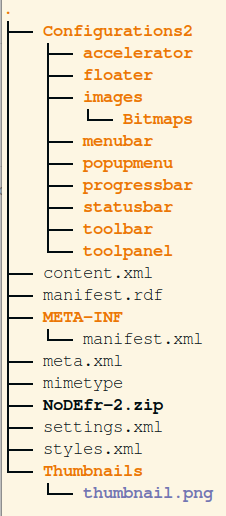
\includegraphics[width=4cm]{arborescence}
    \caption{Arborescence du contenu de l'archive contenant le fichier "NoDEfr-2.ods" }
    \label{fig:mesh1}
\end{figure}



%%%%%%%%%%%%%%%%%%%%%%%%%%%%%%%%%%%%%%%%%%%%%%%%%%%%%%%%%%%%%%%%%%%%%%%%%%%%%%%%%%%%%%%%%%%%%%%%%%%%%%%%%%%%%%%%%%%%%%%%%%%%%%%%%%%%%%%%%%%%%%%%%%%%%%%%%%%%%%%%%%%%%%%%%%%%%%%%%%%%%%%%%%%%%%%%%%%%%%%%%%%%%%%%
\chapter{Identification des solutions}

Nous avons pensé à deux solutions possibles pour résoudre le problème :
\begin{enumerate}
    \item Utilisation de Python
    \item Utilisation du XSLT
\end{enumerate}

\section{Python}
Au début de notre réflexion, nous avions mal cerné ce qu'était "réellement" un fichier ODS.\\
Nous nous sommes donc orientées vers le langage Python. Le programme que nous avons premièrement implémenté fonctionnait de la façon suivante :
\begin{itemize}
    \item Lecture et extraction des données de l'ods
    \item Une fonction "creationRacine" qui crée la racine de l'arbre
    \item Une fonction "creationFils" qui permet de créer des fils qui seront non pas des attributs mais des sous-classes de la classe traitée 
    \item Une fonction "obtenirValeurCellule" qui permet de récupérer les données contenues dans les cellules d'une même ligne en commençant par la cellule passée en entrée.
    \item Une fonction "contenuSheetSecondaire" qui va venir chercher les propriétés de la classe voulue dans la feuille qui lui correspond.
\end{itemize}

\vspace{0.5cm}
Ceci est juste une brève explication du contenu puisqu'il ne s'agit pas de l'implémentation retenue.\\

\underline{Inconvénients}\\
Cette méthode soulève des inconvénients. En effet, Python n'est pas un langage conçu initiallement pour traiter du XML. Il peut en produire à l'aide de bibliothèque importée mais ce n'est pas sa fonction principale ce qui nous a crée de nombreux problèmes (accents, espace et ponctuation mal interprétés). De plus, l'accès aux noeuds est "artifiel". Nous parcourons le fichier ods de manière "barbare", en créant nous même les noeuds à l'aide des cellules du tableau. \\

En conclusion, il répond à notre besoin mais n'est pas le langage optimal.


\section{XSLT}
Le langage XSLT (eXtensible Stylesheet Language Transformation) est décrit comme une application XML spécifiant des règles de transformation d’un document en un autre. Une feuille de style XSLT compare les éléments d’un document XML aux modèles de la feuille de style.\\

Cette définition donne directement la solution à notre problème.\\
De plus, entre temps, nous avons compris ce qui se cache derrière un document ODS. Comme décrit page 4, nous avons  notre disposition un fichier "content.xml" qui nous permet d'appliquer directement le langage XSLT pour produire le fichier XML que nous souhaitons.


%%%%%%%%%%%%%%%%%%%%%%%%%%%%%%%%%%%%%%%%%%%%%%%%%%%%%%%%%%%%%%%%%%%%%%%%%%%%%%%%%%%%%%%%%%%%%%%%%%%%%%%%%%%%%%%%%%%%%%%%%%%%%%%%%%%%%%%%%%%%%%%%%%%%%%%%%%%%%%%%%%%%%%%%%%%%%%%%%%%%%%%%%%%%%%%%%%%%%%%%%%%%%%%%
\chapter{Choix et implémentation d'une solution en la décrivant}
Suite à une réflexion sur les différents langages, nous avons opté pour l'utilisation du XSLT.\\
Voici ci-dessous la description détaillée de notre implémentation.
 
\section{Description de notre implémentation}

Tout le code est disponible en annexe pour rendre l'explication plus lisible.

%%%%%%%%%%%%%%%%%%%%%%%%%%%%%%%%%%%%%%%%%%%%%%%%%%%%%%%%%%%%%%%%%%%%%%%%%%%%%%%%%%%%%%
\subsection{Attributs du stylesheet [Annexe 7.1]} 
Un .ods est une extension de fichier utilisé par OpenDocument. OpenDocument est un format de fichier XML compressé au format ZIP pour les feuilles de calcul, les graphiques, les présentations et les documents de traitement de texte.\\ 
OpenDocument est la désignation d'usage d'une norme dont l'appellation officielle est OASIS Open Document Format for Office Applications.\\

Tous ces liens (issus de oasis) sont nécessaires pour le traitement et l'accès aux cellules du fichier.




%%%%%%%%%%%%%%%%%%%%%%%%%%%%%%%%%%%%%%%%%%%%%%%%%%%%%%%%%%%%%%%%%%%%%%%%%%%%%%%%%%%%%%
\subsection{Accès au noeud de l'arbre "Classes" [Annexe 7.2]}

Nous nous positionons à la racine de notre document "content.xml".\\

Le contenu du fichier qui nous intéresse commence à la ligne 727 par :
\begin{lstlisting}[language=XSLT]
<table:table table:name="Classes" table:style-name="ta2">
\end{lstlisting}

Ainsi, après analyse du fichier, nous recherchons tous les descendants qui ont pour balise \lstinline{table:table} avec un filtre pour ne sélectionner que ceux dont le nom est "Classes". En effet, les autres correspondent aux "relations" que nous traiterons que dans un second temps.\\

Par la suite, nous nous intéressons aux balises \lstinline{table:table-row} qui correspondent à chaque ligne du document.
Dans un premier temps, la première ligne est sautée (il s'agit de l'entête du la feuille traitée) puis \lstinline{following-sibling::table:table-row[1]} permet de traiter tous les noeuds frères suivants.



%%%%%%%%%%%%%%%%%%%%%%%%%%%%%%%%%%%%%%%%%%%%%%%%%%%%%%%%%%%%%%%%%%%%%%%%%%%%%%%%%%%%%%
\subsection{Extraction des données de la feuille "Classes" [Annexe 7.3] }

Lors du parcours du document à la recherche de \lstinline{.//table:table[@table:name='Classes']/table:table-row/}, le template \lstinline{match="table:table-row"} est appliqué.\\

Dans un soucis de récupération du contenu des feuilles de calcul secondaires, autrement appelées les "Relations des Classes", l'identifiant de la classe doit être conservé. Ainsi, la variable \lstinline{idClasse} stocke, à partir du noeud courant, le contenu de la première cellule de la ligne.\\

Pour la suite, en accord avec le schéma XSD, tout le contenu des cellules est récupéré individuellement et placé dans des balises spécifiques.\\
A partir du noeud courant, c'est-à-dire \lstinline{table:table[@table:name='Classes']/table:table-row/}, le contenu des cellules se trouve dans une balise appelée \lstinline{<table:table-cell/<text:p>}. En précisant le numéro de la cellule, nous pouvons en extraire l'intérieur.\\

Dans un deuxième temps, avant de passer au traitement de la classe suivante, nous souhaitons extraire les informations complémentaires liées à la classe en question.\\
Pour ce faire, il faut accéder à une autre table. Ceci est traité avec l'instruction suivante : \lstinline{<xsl:apply-templates select="//table:table[@table:name=\$idClasse]"/>}.
Voici la raison pour laquelle nous avons crée une variable qui permet de récupérer l'identifiant de la classe.


%%%%%%%%%%%%%%%%%%%%%%%%%%%%%%%%%%%%%%%%%%%%%%%%%%%%%%%%%%%%%%%%%%%%%%%%%%%%%%%%%%%%%%
\subsection{Extraction des données des feuilles secondaires [Annexe 7.4] }

Le but de ce template est de récupérer les informations liées aux classes traitées. \\
A chaque fois qu'une ligne de la table "Classes" est extraite, ce template est appelé avec comme filtre \lstinline{[@table:name=\$idClasse]} qui permet de s'intéresser à la table de la classe en question.\\

Pour chaque ligne du tableau, nous récupérons le contenu des cellules en précisant le nom de la balise en accord avec le schéma XSD.\\
L'instruction \lstinline{following-sibling::table:table-row[1]} permet de récupérer tous les noeuds frères, donc toutes les lignes de la feuille en question à l'exception de l'entête. \\
Dans un premier temps, nous récupérons le contenu des celulles comme dans la partie précédente.\\

Cependant, nous nous sommes aperçues, dans un second temps, de l'absence de certaines balises, et même de décalage entre les valeurs des balises et les balises elles-mêmes.\\
Cette erreur provient du fait que dans le fichier "content.xml", lorsqu'une cellule est vide, celle-ci n'est pas explicitement écrite. Nous retrouvons souvent dans le fichier \lstinline{<table:table-cell table:style-name="ce67" table:number-columns-repeated="3"/>}. L'attribut \lstinline{table:number-columns-repeated="3"} indique que les deux celulles suivantes ainsi que celle en question contiennent les mêmes valeurs. Dans notre cas, ceci implique que les cellules sont vides, sauf lorsqu'il s'agit des balises de cardinalité.\\

Il a donc fallu prendre en compte cette notation. En étudiant le fichier, cet attibut n'est présent que pour les balises suivantes : regleDeContenu, raffine, exemple, note, cardinaliteMinimale, cardinaliteMaximale et raison.\\
De plus, cet attribut possède des valeurs maximum différentes en fonction des balises.\\
Ainsi :
\begin{itemize}
    \item \lstinline{regleDeContenu} prend des valeurs allant 1 à 4. \\ A titre d'exemple, 4 signifie que lui même et les trois prochaines colonnes sont vides.\\ Lorsque le programme arrive sur le traitement de la colonne 6 "regleDeContenu", il stocke dans la variable appelée "répétition" l'attribut \lstinline{table:number-columns-repeated}.\\
    Par la suite, un \lstinline{<xsl:choose>} est implémenté qui correspond à un choix en fonction de la valeur de la variable "répétition".\\
    Une fois dans le \lstinline{<xsl:when test="\$repetition=...">}, de nouveaux templates sont appelés pour récupérer les valeurs des celulles. \\
    Voici un exemple : 
    \begin{lstlisting}[language=XSLT]
<xsl:call-template name="regleDeContenu">
    <xsl:with-param name="j" select="6"/>
</xsl:call-template>
<xsl:variable name="repetition">
    <xsl:value-of select="number(.//table:table-cell[6]/@table:number-columns-repeated)"/>
</xsl:variable>

<xsl:choose>
    <xsl:when test="$repetition=4">
        <xsl:call-template name="raffine">
            <xsl:with-param name="j" select="6"/>
        </xsl:call-template>
        <xsl:call-template name="exemple">
            <xsl:with-param name="j" select="6"/>
        </xsl:call-template>
        <xsl:call-template name="note">
            <xsl:with-param name="j" select="6"/>
        </xsl:call-template>
        <xsl:call-template name="card_temp">
            <xsl:with-param name="i" select="7"/>
        </xsl:call-template>
    </xsl:when>
    \end{lstlisting}
    qui, au début, appelle le template pour la récupération du contenu de la balise éregleDeContenu" : 
    \begin{lstlisting}[language=XSLT]
    <xsl:template name="regleDeContenu">
        <xsl:param name="j"/>
            <xsl:element name="regleDeContenu">
                <xsl:value-of select=".//table:table-cell[$j]/text:p"/>
            </xsl:element>
    </xsl:template>
    \end{lstlisting}
    Le même procédé est réalisé pour les autres balises.
    \item \lstinline{raffine_temp} prend des valeurs allant 1 à 3.
    \item \lstinline{exemple_temp} prend des valeurs allant 1 à 2.
    \item \lstinline{note_temp} prend des valeurs allant 1 à 3.
    \item \lstinline{card_temp} prend des valeurs allant 1 à 2.
\end{itemize}

\vspace{0.5cm}
Dans l'annexe, seulement un exemple est présent par peur d'alourdir le fichier pdf.\\



%%%%%%%%%%%%%%%%%%%%%%%%%%%%%%%%%%%%%%%%%%%%%%%%%%%%%%%%%%%%%%%%%%%%%%%%%%%%%%%%%%%%%%%%%%%%%%%%%%%%%%%%%%%%%%%%%%%%%%%%%%%%%%%%%%%%%%%%%%%%%%%%%%%%%%%%%%%%%%%%%%%%%%%%%%%%%%%%%%%%%%%%%%%%%%%%%%%%%%%%%%%%%%%%
\chapter{Validation avec le XSD ?}

Le XML produit doit être compatible avec le schéma XSD produit par l'équipe 1.

\subsection{Suppression des balises vides [Annexe 7.5]}

Quand nous avons voulu valider notre XML à l'aide du schéma XSD, nous avons rencontré un problème : les éléménets vides (\texttt{<balise/>}) étaient interprété comme des chaînes de caractères vides, ce qui n'était pas accepté par le schéma XSD. \\

En accord avec l'équipe 1, nous avons décidé de supprimer les balises vides. Pour cela, nous avons utilisé un deuxième programme XSLT prenant en entrée le XML produit jusque là (NoDEfr-2.1.xml) et produisant en sortie un nouveau fichier XML : NoDEfr-2.2.xml.\\

Ce second programme permet de recopier à l'identique le premier XML tout en supprimant tous les éléments vides ayant pour balise : definition, coDomaine, regleDeContenu, raffine, exemple, note ou raison.\\

\subsection{Problème de référence des classes [Annexe 7.6]}

Une fois le problème des éléments vides réglé, le XML n'était toujours pas validé à cause d'un problème de référence. En effet, lorsqu'une classe est décrite, l'un de ses attributs est "sousClasseDe" qui fait référence à d'autres classes. Dans le XSD, l'attribut "identifiant" d'une classe est de type \lstinline{xsd:ID} est les classes appartenant à l'attribut "sousClasseDe" sont des \lstinline{xsd:IDREF} (ou \lstinline{xsd:IDREFS} s'il y en a plusieurs), il est donc invalide d'avoir en attribut "sousClasseDe" une classe qui n'a pas été déclaré au préalable dans le XML. \\

Une solution envisagée pour ce problème a été de créer un sommaire au début du premier XML contenant les liste des classes, leur identifiant et leur position (allant de 1 à 29). Ce sommaire serait utilisé dans le second programme XSLT. Pour chaque classe, le programme vérifirait que les classes de l'attribut "sousClasseDe" ont été déclarées au préalable (la classe de l'attribut "sousClasseDe" se trouve plus haut dans le sommaire que la classe traitée). Si la classe n'a pas été déclarée, elle serait traitée à la fin seulement. \\
Le problème lié à cette solution est l'impossibilité de faire varier des variables dans un programme XSLT. \\ 
Après plusieurs tentatives de mise en place de solutions, nous avons conclu que la complexité du problème et de sa solution nous dépassait et avons pris la décision de ne pas valider le XML. Cette décision était notamment soutenue par le fait que l'erreur ne concernait que 5 classes. \\


%%%%%%%%%%%%%%%%%%%%%%%%%%%%%%%%%%%%%%%%%%%%%%%%%%%%%%%%%%%%%%%%%%%%%%%%%%%%%%%%%%%%%%%%%%%%%%%%%%%%%%%%%%%%%%%%%%%%%%%%%%%%%%%%%%%%%%%%%%%%%%%%%%%%%%%%%%%%%%%%%%%%%%%%%%%%%%%%%%%%%%%%%%%%%%%%%%%%%%%%%%%%%%%%
\chapter{Conclusion}

%en portant un regard critique sur votre travail

Nous partions de données issues d'un document ods. Premier point qu'il nous a fallu eclaircir : qu'est-ce que réellement un fichier ods ?\\
En effet, notre première erreur formatrice fut de partir en implémentation python en ne sachant pas qu'un ods est constitué de XML. Le Python nous semblait être le langage le plus approprié pour extraire les données d'un ods puis former un XML à partir de ces données.\\

Cependant, lors du point effectué en cours, nous avons vite compris que nous étions parties dans la mauvaise direction. Le XSLT est bien sûr le langage à utiliser.\\

Nous avons pu repenser notre façon de voir les choses et repartir sur de nouvelles bases.\\

Cependant, a posteriori, le traitement des cellules vides aurait été bien plus facile à traiter en Python qu'en XSLT. En effet, en Python, les cellules vides sont récupérées comme des cellules ayant du contenu. En XSLT, les balises n'ayant pas de texte ne sont pas nécessairement explicites. Un attribut dans la balise précedente permet de le souligner. Cette façon de contruire un XML nous a obligé à implémenter de nouveaux templates.\\

Le fait d'avoir réalisé ce projet en deux langages nous a permis de voir les avantages et inconvénients et également de se rendre compte que pour aboutir au même résultat une méthode est plus efficace qu'une autre.



%%%%%%%%%%%%%%%%%%%%%%%%%%%%%%%%%%%%%%%%%%%%%%%%%%%%%%%%%%%%%%%%%%%%%%%%%%%%%%%%%%%%%%%%%%%%%%%%%%%%%%%%%%%%%%%%%%%%%%%%%%%%%%%%%%%%%%%%%%%%%%%%%%%%%%%%%%%%%%%%%%%%%%%%%%%%%%%%%%%%%%%%%%%%%%%%%%%%%%%%%%%%%%%%
\chapter{Annexe}

\section{Attributs du stylesheet}
\begin{lstlisting}[language=XSLT]
xmlns:xsl="http://www.w3.org/1999/XSL/Transform" version="2.0"
xmlns:office="urn:oasis:names:tc:opendocument:xmlns:office:1.0" 
xmlns:style="urn:oasis:names:tc:opendocument:xmlns:style:1.0" 
xmlns:text="urn:oasis:names:tc:opendocument:xmlns:text:1.0" 
xmlns:table="urn:oasis:names:tc:opendocument:xmlns:table:1.0"
xmlns:draw="urn:oasis:names:tc:opendocument:xmlns:drawing:1.0"
xmlns:fo="urn:oasis:names:tc:opendocument:xmlns:xsl-fo-compatible:1.0" 
xmlns:xlink="http://www.w3.org/1999/xlink" 
xmlns:dc="http://purl.org/dc/elements/1.1/"
xmlns:meta="urn:oasis:names:tc:opendocument:xmlns:meta:1.0" 
xmlns:number="urn:oasis:names:tc:opendocument:xmlns:datastyle:1.0"
xmlns:svg="urn:oasis:names:tc:opendocument:xmlns:svg-compatible:1.0"
xmlns:chart="urn:oasis:names:tc:opendocument:xmlns:chart:1.0"
xmlns:dr3d="urn:oasis:names:tc:opendocument:xmlns:dr3d:1.0"
xmlns:math="http://www.w3.org/1998/Math/MathML"
xmlns:form="urn:oasis:names:tc:opendocument:xmlns:form:1.0"
xmlns:script="urn:oasis:names:tc:opendocument:xmlns:script:1.0"
xmlns:ooo="http://openoffice.org/2004/office"
xmlns:ooow="http://openoffice.org/2004/writer"
xmlns:oooc="http://openoffice.org/2004/calc"
xmlns:dom="http://www.w3.org/2001/xml-events"
xmlns:xforms="http://www.w3.org/2002/xforms"
xmlns:xsd="http://www.w3.org/2001/XMLSchema"
xmlns:xsi="http://www.w3.org/2001/XMLSchema-instance" 
office:version="1.0">
\end{lstlisting}


\section{Premier "xsl:template"}
\begin{lstlisting}[language=XSLT]
<xsl:template match="/">
    <xsl:element name="Modele">
        <xsl:apply-templates select=".//table:table[@table:name='Classes']/table:table-row/following-sibling::table:table-row[1]"/>
    </xsl:element>
</xsl:template>
\end{lstlisting}

\section{Second "xsl:template"}
\begin{lstlisting}[language=XSLT]
<xsl:template match="table:table-row">
    <xsl:variable name="idClasse">
        <xsl:value-of select=".//table:table-cell[1]/text:p"/>
    </xsl:variable>
    <xsl:element name="classe">
        <xsl:element name="identifiant">
            <xsl:value-of select=".//table:table-cell[1]/text:p"/>
        </xsl:element>
        <xsl:element name="nom">
            <xsl:value-of select=".//table:table-cell[2]/text:p"/>
        </xsl:element>
        <xsl:element name="definition">
            <xsl:value-of select=".//table:table-cell[3]/text:p"/>
        </xsl:element>
        <xsl:element name="sousClasseDe">
            <xsl:value-of select=".//table:table-cell[4]/text:p"/>
        </xsl:element>
        <xsl:element name="note">
            <xsl:value-of select=".//table:table-cell[5]/text:p"/>
        </xsl:element>
        <xsl:apply-templates select="//table:table[@table:name=$idClasse]"/>
    </xsl:element>
</xsl:template>
\end{lstlisting}


\section{Troisième "xsl:template"}
\begin{lstlisting}[language=XSLT]
<xsl:template match="table:table">
    <xsl:for-each select=".//table:table-row/following-sibling::table:table-row[1]">
        <xsl:element name="relation">
            <xsl:attribute name="identifiant">
                <xsl:value-of select=".//table:table-cell[1]/text:p"/>
            </xsl:attribute>
            <xsl:element name="nom">
                <xsl:value-of select=".//table:table-cell[2]/text:p"/>
            </xsl:element>
            <xsl:element name="definition">
                <xsl:value-of select=".//table:table-cell[3]/text:p"/>
            </xsl:element>
            <xsl:element name="indicateurLinguistique">
                <xsl:value-of select=".//table:table-cell[4]/text:p"/>
            </xsl:element>
            <xsl:element name="coDomaine">
                <xsl:value-of select=".//table:table-cell[5]/text:p"/>
            </xsl:element>
            
            <xsl:call-template name="regleDeContenu">
                <xsl:with-param name="j" select="6"/>
            </xsl:call-template>
            <xsl:variable name="repetition">
                <xsl:value-of select="number(.//table:table-cell[6]/@table:number-columns-repeated)"/>
            </xsl:variable>

            <xsl:choose>
                <xsl:when test="$repetition=4">
                    <xsl:call-template name="raffine">
                        <xsl:with-param name="j" select="6"/>
                    </xsl:call-template>
                    <xsl:call-template name="exemple">
                        <xsl:with-param name="j" select="6"/>
                    </xsl:call-template>
                    <xsl:call-template name="note">
                        <xsl:with-param name="j" select="6"/>
                    </xsl:call-template>
                    <xsl:call-template name="card_temp">
                        <xsl:with-param name="i" select="7"/>
                    </xsl:call-template>
                </xsl:when>
                <xsl:when test="$repetition=3">
                    <xsl:call-template name="raffine">
                        <xsl:with-param name="j" select="6"/>
                    </xsl:call-template>
                    <xsl:call-template name="exemple">
                        <xsl:with-param name="j" select="6"/>
                    </xsl:call-template>
                    <xsl:call-template name="note_temp">
                        <xsl:with-param name="i" select="7"/>
                    </xsl:call-template>                    
                </xsl:when>
                <xsl:when test="$repetition=2">
                    <xsl:call-template name="raffine">
                        <xsl:with-param name="j" select="6"/>
                    </xsl:call-template>
                    <xsl:call-template name="exemple_temp">
                        <xsl:with-param name="i" select="7"/>
                    </xsl:call-template>
                </xsl:when>
                <xsl:otherwise>
                    <xsl:call-template name="raffine_temp">
                        <xsl:with-param name="i" select="7"/>
                    </xsl:call-template>                    
                </xsl:otherwise>
            </xsl:choose>

        </xsl:element>
    </xsl:for-each>        
</xsl:template> 
\end{lstlisting}

\section{Deuxième XSLT "xsl:template"}
\begin{lstlisting}[language=XSLT]
<?xml version="1.0" encoding="UTF-8" standalone="yes"?>
<xsl:stylesheet version="2.0"
    xmlns:xsl="http://www.w3.org/1999/XSL/Transform">
    <xsl:output indent="yes" encoding="UTF-8"/>
    
    <xsl:strip-space elements="*"/>

    <xsl:template match="/">
        <xsl:apply-templates/>
    </xsl:template>

    <xsl:template match="Modele">
        <xsl:copy>
            <xsl:apply-templates select=".//classe"/>
        </xsl:copy>
    </xsl:template>

    <xsl:template match="classe">
        <xsl:if test="string(@identifiant)">
            <xsl:copy>
                <xsl:copy-of select="@*"/>
                <xsl:copy-of select="./*[name()!='relation']"/>
                <xsl:apply-templates select=".//relation"/>
            </xsl:copy>
        </xsl:if>
    </xsl:template>

    <xsl:template match="relation">
        <xsl:if test="string(@identifiant)">
            <xsl:copy>
                <xsl:copy-of select="@*"/>
                <xsl:for-each select="./*">
                    <xsl:choose>
                        <xsl:when test="((name()='definition') or
                                        (name()='coDomaine') or 
                                        (name()='regleDeContenu') or
                                        (name()='raffine') or 
                                        (name()='exemple') or
                                        (name()='note') or
                                        (name()='raison')) and 
                                        (string()='')">
                        </xsl:when>
                        <xsl:otherwise>
                            <xsl:copy-of select="@*"/>
                            <xsl:copy-of select="."/>
                        </xsl:otherwise>
                    </xsl:choose>
                </xsl:for-each>
            </xsl:copy>
        </xsl:if>
    </xsl:template>

</xsl:stylesheet>

\end{lstlisting}

\section{Validation du XML}
\begin{lstlisting}[language=bash]
NoDEfr-2.2.xml:148: element sousClasseDe: Schemas validity error : Element 'sousClasseDe': 'RC0050,' is not a valid value of the atomic type 'xs:IDREF'.
NoDEfr-2.2.xml:148: element sousClasseDe: Schemas validity error : Element 'sousClasseDe': 'RC0050, RC0030' is not a valid value of the list type 'xs:IDREFS'.
NoDEfr-2.2.xml:607: element sousClasseDe: Schemas validity error : Element 'sousClasseDe': 'RC0050,' is not a valid value of the atomic type 'xs:IDREF'.
NoDEfr-2.2.xml:607: element sousClasseDe: Schemas validity error : Element 'sousClasseDe': 'RC0050, RC0030' is not a valid value of the list type 'xs:IDREFS'.
NoDEfr-2.2.xml:717: element sousClasseDe: Schemas validity error : Element 'sousClasseDe': 'RC0100,' is not a valid value of the atomic type 'xs:IDREF'.
NoDEfr-2.2.xml:717: element sousClasseDe: Schemas validity error : Element 'sousClasseDe': 'RC0100, RC0030' is not a valid value of the list type 'xs:IDREFS'.
NoDEfr-2.2.xml fails to validate
\end{lstlisting}


\end{document}